%% -*- mode: latex; mode: reftex; mode: flyspell; TeX-master: "top.tex"; -*-

\vspace{-3mm}

The input to our approach is a series of $T$
images $\mathcal{I} = \{I_1, \ldots, I_t, \ldots,
I_T\}$ from which we extract $K$ nucleus
detections $d_t^k$.  The tracking step described
in Sec.~\ref{sec:tracking} associates valid
detections across time steps while rejecting
spurious detections. Since each neuron contains
only one nucleus, there is a one-to-one mapping
between each valid nucleus detection $c_t^i$ and a
neuron $X_t^i$.  Thus, the tracking task is to
provide a set of neuron detections $\mathcal{X}^i
= \{X_{a}^i,\ldots,X_t^i,\ldots,X_{b}^i \}$
defining an individual neuron $i$ from time $t=a$
to $t=b$.  As depicted in Fig.~\ref{fig:notation},
each neuron detection $X_t^i$ is composed of a
nucleus $c_t^i$, a soma $s_t^i$, a set of $J$
neurites $\{n_t^{i,1}, \ldots, n_t^{i,j}, \ldots,
n_t^{i,J} \}$, and a set of $L$ filopodia
associated with each neurite $F_t^{i,j} =
\{f_t^{i,j,1},\ldots,f_t^{i,j,l},\ldots,f_t^{i,j,L}
\}$ so that $N_t^i = \{( n_t^{i,1},F_t^{i,1}),
\ldots,(n_t^{i,j},F_t^{i,j}) \}$.  Thus, a
complete neuron $i$ at time step $t$ is described
by $X_t^i = \{ c_t^i, s_t^i, N_t^i \}$.


\vspace{-3mm}
\subsection{Nuclei and Somata Detection and Segmentation}
\vspace{-2mm}
\label{sec:detection}
%% \vspace{-2mm}
The first step in our approach is to extract a set
of nucleus detections $\{d^1,\ldots,d^K\}$ over
the image series. We worked with two-channel
images where the cytoskeleton is marked with
Lifeact-GFP and nuclei are marked with
NLS-mCherry. The nuclei can be reliably detected
and segmented by simply thresholding the
NLS-mCherry channel and performing a morphological
filling operation.  Alternatively, one could apply
a fast machine learning detector such as the one
in~\cite{Smith09}.


Using the nuclei as seed points, somata are
segmented as follows.  A list of pixels
neighboring the current soma segmentation is
maintained.  At each iteration, the neighbor with
the smallest weighted distance to the centroid of
the seed nucleus detection $D = \lambda || u -
d^k|| + |I(u) - \hat{I}(d^k)|$ is added to the
soma so long as $D < Y$, where $u$ is a location
in the image, $I(u)$ is the pixel intensity at
that location, $\hat{I}(d^k)$ is the mean
intensity of detection $d^k$, and $Y$ is a
threshold.


\vspace{-3mm}
\subsection{Efficient Tracking of Nucleus Detections}
\label{sec:tracking}
\vspace{-2mm}

The tracking algorithm searches through the full
set of nuclei detections and iteratively
associates the most similar pairs of detections,
returning lists of valid detections corresponding
to each neuron $\mathcal{X}^i$.  This is
accomplished by constructing a graph
$\mathcal{G}=(\mathcal{D},\mathcal{E})$ where each
node $d^k_t \in \mathcal{D}$ corresponds to a
detection.  For each detection $d^k_t$ in time
step $t$, edges $e \in \mathcal{E}$ are formed
between $d^k_t$ and all past and future detections
within a time window $W$.  A weight $w_e$ is
assigned to each edge $e^{k,l}$ connecting $d^k_t$
and $d^l_t$. The weight $w_e$ relates to spatial
distances, temporal distances, and a shape
measure: $w_{e} = \alpha || d^k_{t1} - d^l_{t2} ||
+ \beta |t1 - t2| + \gamma f(\nu^k_{t1},
\nu^l_{t2})$, where $\nu^k$ is a shape feature
vector containing $d^k_t$'s area, perimeter, mean
intensity, and major and minor axis lengths of a
fitted ellipse. $f$ evaluates differences between
a feature $a$ extracted from $d^k_t$ and $d^l_t$
as $f(a^k,a^l) = {|a^k - a^l|}/{|a^k + a^l|}$.
The tracking solution corresponds to a set of
edges $\mathcal{E'} \subset \mathcal{E}$ with
maximal edge weight $Q$ that forms a set of
disconnected tracks $\mathcal{T}$ and minimizes
the cost function $\sum_{e \in \mathcal{T}} w_e$.

To minimize this cost function, we adopt a greedy
selection algorithm, summarized in
Fig.~\ref{fig:greedytracking}, that iteratively
selects an edge with minimum cost $\hat w_e$ and
adds it to the set $\mathcal{L}$ removing future
and past connections from the detections $e^{k,l}$
connects.  The algorithm iterates until the
minimum cost $\hat w_e$ is greater than a
threshold $Q$.  Each track $i$ is then associated
with a neuron identity $\mathcal{X}^i$.




%----------------------------------------------------------------------------
\begin{figure}[t]
  \begin{center}
       \begin{tabular}{@{\hspace{-1mm}}c}
        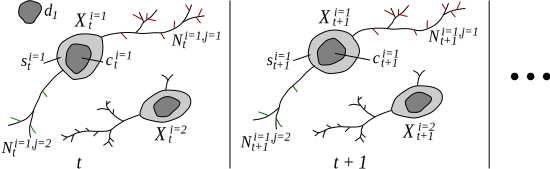
\includegraphics[width = 87mm] {images/neurondrawing.pdf}\\ [-2.4ex]
       \end{tabular} 
    \caption{ \footnotesize Neuron tracking
      notation.  At time $t$ a neuron $i$
      detection $X_t^i = \{ c_t^i, s_t^i, N_t^i
      \}$ contains a nucleus $c_t^i$, a soma
      $s_t^i$, and a set of neurite-filopodia
      tuples $N_t^i = \{( n_t^{i,1},F_t^{i,1}),
      \ldots,(n_t^{i,j},F_t^{i,j}), \ldots,
      (n_t^{i,J},F_t^{i,J}) \}$ which contains $J$
      neurites and their associated filopodia
      shown in red for $j=1$ and green for
      $j=2$. A spurious nucleus detection $d_1$ is
      also shown.  A neuron $i$ is defined by a
      time-series of neuron detections
      $\mathcal{X}^i =
      \{X_{a}^i,\ldots,X_t^i,\ldots,X_{b}^i \}$.
      The tracking returns a set $\mathcal{X}^i$
      for each neuron. }
    \label{fig:notation}
  \end{center}
\vspace{-8mm}
\end{figure}
%% by linking nucleus detections  and ``growing'' the
%%         neuron from the nucleus seed
%----------------------------------------------------------------------------







\vspace{-3mm}
\subsection{Neuron Segmentation and Neurite Tree Extraction}
\label{sec:segmentation}
\vspace{-2mm} Given an image $I_t$ and the set of
somata present in it $S_t=\{s_t^1 \dots s_t^m \}$,
our goal is to associate to each pixel $u$ a label
$J_t(u)$ that indicates to which neuron (soma) it
belongs, if any.  The probability of $J_t(u)$ can
be deduced using Bayes' rule,
\begin{equation}
  \label{eq:bayes}
  P(J_t(u)=i|S_t,I_t) = \frac{P(S_t,I_t| J_t(u)=i)}{\sum_{\eta=1}^m P(S_t,I_t|J_t(u)=\eta)},
\end{equation}
\noindent where we assume a uniform distribution
on $P(J_t(u))$.  The numerator is modeled as the
probability of the path $L$ that connects
maximally pixel $u$ to soma $s_t^i$, $ P(S_t,I_t|
J_t(u)=i) = \max_{L:u\rightarrow s_t^i}
\prod_{\{l_{r}\} \in L } P(I_t(r)|l_{r}),$ where
$l_{r}$ are indicator variables for the locations
forming the path $L$.  We chose this model since
it produces connected components and an optimal
maxima can be found by minimizing its negative
likelihood using Dijkstra's shortest path.

To optimize this function, we map the image $I_t$
to a graph $\mathcal{G}_t^i = (V,E)$ whose
vertices $u$ are the pixels in $I_t$ and whose
directed edges $e_{r,v}$ connect each pixel to its
four neighbors.  We assign to each edge a weight
$w_{r,v} = -log P(I_t(v)|v)$.  $P(I_t(v)|v)$
represents the probability that a neurite
traverses a node $v$.  It is obtained by applying
a sigmoid function to the output of the tubularity
filter of~\cite{Frangi98}.  The parameters of the
sigmoid function are estimated using maximum
likelihood. Finally, we define the set of neurite
pixels $U_n^t$ as those that connect to any soma
with a higher probability than $\epsilon$.  We
predict their labels as the ones that maximize
Eq.~\ref{eq:bayes}.  The set of pixels associated
to neuron $X_t^i$ is the union of the neurites and
the soma associated with $i$, $ U_i^t = \{u \in
U_n^t | J_t(u) = i\} \cup s_t^i$. To reduce the
neurite segmentation to a tree, we skeletonize the
neuron and define as root node the pixel of the
skeleton closest to the centroid of the nucleus.
We instantiate a Minimum Spanning Tree from the
root and create a neurite tree whenever the
spanning tree exits the soma.




\subsection{Neurite Tracking and Filopodia Detection}
\label{sec:neurite}
\vspace{-2mm} The identity of neurites is tracked
across the frames of the time-lapse videos by
applying the algorithm described in
Sec~\ref{sec:tracking}, but using the centroids of
the neurite trees instead of the centroids of
nuclei, with the additional constraint that edges
may only exist between neurites that emanate from
the same soma.  Filopodia are detected by starting
at each leaf node in a neurite and traversing the
tree until a branch point is reached. If the
distance traversed is less than a threshold $T_f$,
the traversed locations are considered to be
filopodia.


%----------------------------------------------------------------------------
\begin{figure}[t]
  \centering
       \begin{tabular}{@{\hspace{-1mm}}c@{}}
        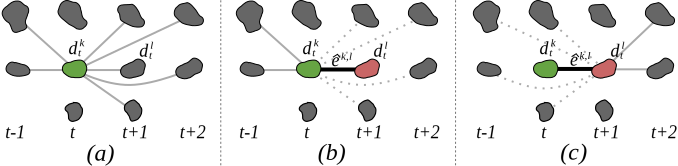
\includegraphics[width = 85mm] {images/greedytracking.pdf}\\ [-2.4ex]
       \end{tabular} 
    \caption{ \footnotesize Efficient tracking by
      association.  {\em (a)} A graph is built by
      fully connecting each detection to all
      future and past detections within a time
      window $W$.  In this simplified diagram,
      only $d^k_t$'s edges are shown and
      $W$=2. {\em (b)} Each iteration, the edge
      $\hat{e}^{k,l}$ with minimum cost
      $\hat{w}_e$ is added to $\mathcal{E}'$.
      Edges connecting $d^k_t$ to future
      detections are removed from $\mathcal{E}$.
      {\em (c)} Edges connecting $d^l_t$ to the
      past are removed from $\mathcal{E}$.  The
      process is repeated until $\hat w_e > Q$. }
    \label{fig:greedytracking}
%\vspace{-4mm}
\end{figure}
%----------------------------------------------------------------------------


%%----------------------------------------------------------------------------
%\begin{figure}[t]
%  \centering
%       \begin{tabular}{@{\hspace{-1mm}}c@{}}
%        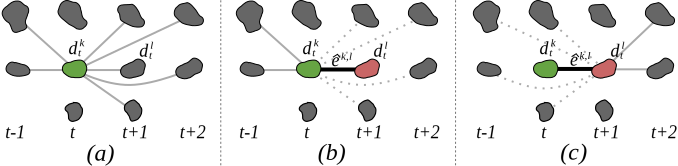
\includegraphics[width = 85mm] {images/greedytracking.pdf}\\ [-2.4ex]
%       \end{tabular} 
%    \caption{ \footnotesize Efficient tracking by association.  {\em  (a)} A graph is
%	built where each detection is fully connected to all future and past detections 
%within  a time  window  $W$.  In this diagram, only  $d^k_t$'s edges  are
%        shown and $W$=2. {\em  (b)} Each iteration,  the edge $\hat{e}^{k,l}$
%        with   minimum  cost   $\hat{w}_e$  is  added  to $\mathcal{E}'$.   Edges  connecting
%        $d^k_t$ to  future detections are  removed from $\mathcal{E}$.
%        {\em  (c)} Edges  connecting  $d^l_t$ to  the past  are
%        removed from $\mathcal{E}$.  The process is repeated until $\hat w_e > Q$. }
%    \label{fig:greedytracking}
%\vspace{-4mm}
%\end{figure}
%%----------------------------------------------------------------------------

%%-----------------------------------------------------------------
%\begin{algorithm}[b]
%\caption{Tracking association algorithm}
%\footnotesize
%\begin{algorithmic}[100]
%\STATE Start with an empty set $\mathcal{E}'$.
%\REPEAT
%\STATE Find edge $\hat e^{k,l}$ with minimum cost $\hat w_e$.
%\STATE Add $\hat e^{k,l}$ to $\mathcal{E}'$, linking detections $d^k_{t1}$ and $d^l_{t2}$.
%\STATE Remove $\hat e^{k,l}$ from $\mathcal{E}$.
%\IF {$ t1 < t2 $}
%\STATE Remove edges between $d^k_{t1}$ and {\em future} detections (where $t > t1$) from $\mathcal{E}$
%\STATE Remove edges between $d^l_{t2}$ and {\em past} detections (where $t < t2$) from $\mathcal{E}$
%\ELSE
%\STATE Remove edges between $d^k_{t1}$ and {\em past} detections (where $t < t1$) from $\mathcal{E}$
%\STATE Remove edges between $d^l_{t2}$ and {\em future} detections (where $t > t2$) from $\mathcal{E}$
%\ENDIF
%\UNTIL{$\hat w_e > Q$}
%\end{algorithmic}
%\normalsize
%\label{algo:greedy}
%\end{algorithm}
%%-----------------------------------------------------------------
